\PassOptionsToPackage{unicode=true}{hyperref} % options for packages loaded elsewhere
\PassOptionsToPackage{hyphens}{url}
\PassOptionsToPackage{dvipsnames,svgnames*,x11names*}{xcolor}
%
\documentclass[]{article}
\usepackage{lmodern}
\usepackage{amssymb,amsmath}
\usepackage{ifxetex,ifluatex}
\usepackage{fixltx2e} % provides \textsubscript
\ifnum 0\ifxetex 1\fi\ifluatex 1\fi=0 % if pdftex
  \usepackage[T1]{fontenc}
  \usepackage[utf8]{inputenc}
  \usepackage{textcomp} % provides euro and other symbols
\else % if luatex or xelatex
  \usepackage{unicode-math}
  \defaultfontfeatures{Ligatures=TeX,Scale=MatchLowercase}
\fi
% use upquote if available, for straight quotes in verbatim environments
\IfFileExists{upquote.sty}{\usepackage{upquote}}{}
% use microtype if available
\IfFileExists{microtype.sty}{%
\usepackage[]{microtype}
\UseMicrotypeSet[protrusion]{basicmath} % disable protrusion for tt fonts
}{}
\IfFileExists{parskip.sty}{%
\usepackage{parskip}
}{% else
\setlength{\parindent}{0pt}
\setlength{\parskip}{6pt plus 2pt minus 1pt}
}
\usepackage{xcolor}
\usepackage{hyperref}
\hypersetup{
            pdftitle={Module 11: Recommended Exercises},
            pdfauthor={Emma Skarstein, Daesoo Lee, Stefanie Muff; Department of Mathematical Sciences, NTNU},
            colorlinks=true,
            linkcolor=Maroon,
            filecolor=Maroon,
            citecolor=Blue,
            urlcolor=blue,
            breaklinks=true}
\urlstyle{same}  % don't use monospace font for urls
\usepackage[margin=1in]{geometry}
\usepackage{color}
\usepackage{fancyvrb}
\newcommand{\VerbBar}{|}
\newcommand{\VERB}{\Verb[commandchars=\\\{\}]}
\DefineVerbatimEnvironment{Highlighting}{Verbatim}{commandchars=\\\{\}}
% Add ',fontsize=\small' for more characters per line
\usepackage{framed}
\definecolor{shadecolor}{RGB}{248,248,248}
\newenvironment{Shaded}{\begin{snugshade}}{\end{snugshade}}
\newcommand{\AlertTok}[1]{\textcolor[rgb]{0.94,0.16,0.16}{#1}}
\newcommand{\AnnotationTok}[1]{\textcolor[rgb]{0.56,0.35,0.01}{\textbf{\textit{#1}}}}
\newcommand{\AttributeTok}[1]{\textcolor[rgb]{0.77,0.63,0.00}{#1}}
\newcommand{\BaseNTok}[1]{\textcolor[rgb]{0.00,0.00,0.81}{#1}}
\newcommand{\BuiltInTok}[1]{#1}
\newcommand{\CharTok}[1]{\textcolor[rgb]{0.31,0.60,0.02}{#1}}
\newcommand{\CommentTok}[1]{\textcolor[rgb]{0.56,0.35,0.01}{\textit{#1}}}
\newcommand{\CommentVarTok}[1]{\textcolor[rgb]{0.56,0.35,0.01}{\textbf{\textit{#1}}}}
\newcommand{\ConstantTok}[1]{\textcolor[rgb]{0.00,0.00,0.00}{#1}}
\newcommand{\ControlFlowTok}[1]{\textcolor[rgb]{0.13,0.29,0.53}{\textbf{#1}}}
\newcommand{\DataTypeTok}[1]{\textcolor[rgb]{0.13,0.29,0.53}{#1}}
\newcommand{\DecValTok}[1]{\textcolor[rgb]{0.00,0.00,0.81}{#1}}
\newcommand{\DocumentationTok}[1]{\textcolor[rgb]{0.56,0.35,0.01}{\textbf{\textit{#1}}}}
\newcommand{\ErrorTok}[1]{\textcolor[rgb]{0.64,0.00,0.00}{\textbf{#1}}}
\newcommand{\ExtensionTok}[1]{#1}
\newcommand{\FloatTok}[1]{\textcolor[rgb]{0.00,0.00,0.81}{#1}}
\newcommand{\FunctionTok}[1]{\textcolor[rgb]{0.00,0.00,0.00}{#1}}
\newcommand{\ImportTok}[1]{#1}
\newcommand{\InformationTok}[1]{\textcolor[rgb]{0.56,0.35,0.01}{\textbf{\textit{#1}}}}
\newcommand{\KeywordTok}[1]{\textcolor[rgb]{0.13,0.29,0.53}{\textbf{#1}}}
\newcommand{\NormalTok}[1]{#1}
\newcommand{\OperatorTok}[1]{\textcolor[rgb]{0.81,0.36,0.00}{\textbf{#1}}}
\newcommand{\OtherTok}[1]{\textcolor[rgb]{0.56,0.35,0.01}{#1}}
\newcommand{\PreprocessorTok}[1]{\textcolor[rgb]{0.56,0.35,0.01}{\textit{#1}}}
\newcommand{\RegionMarkerTok}[1]{#1}
\newcommand{\SpecialCharTok}[1]{\textcolor[rgb]{0.00,0.00,0.00}{#1}}
\newcommand{\SpecialStringTok}[1]{\textcolor[rgb]{0.31,0.60,0.02}{#1}}
\newcommand{\StringTok}[1]{\textcolor[rgb]{0.31,0.60,0.02}{#1}}
\newcommand{\VariableTok}[1]{\textcolor[rgb]{0.00,0.00,0.00}{#1}}
\newcommand{\VerbatimStringTok}[1]{\textcolor[rgb]{0.31,0.60,0.02}{#1}}
\newcommand{\WarningTok}[1]{\textcolor[rgb]{0.56,0.35,0.01}{\textbf{\textit{#1}}}}
\usepackage{graphicx,grffile}
\makeatletter
\def\maxwidth{\ifdim\Gin@nat@width>\linewidth\linewidth\else\Gin@nat@width\fi}
\def\maxheight{\ifdim\Gin@nat@height>\textheight\textheight\else\Gin@nat@height\fi}
\makeatother
% Scale images if necessary, so that they will not overflow the page
% margins by default, and it is still possible to overwrite the defaults
% using explicit options in \includegraphics[width, height, ...]{}
\setkeys{Gin}{width=\maxwidth,height=\maxheight,keepaspectratio}
\setlength{\emergencystretch}{3em}  % prevent overfull lines
\providecommand{\tightlist}{%
  \setlength{\itemsep}{0pt}\setlength{\parskip}{0pt}}
\setcounter{secnumdepth}{0}
% Redefines (sub)paragraphs to behave more like sections
\ifx\paragraph\undefined\else
\let\oldparagraph\paragraph
\renewcommand{\paragraph}[1]{\oldparagraph{#1}\mbox{}}
\fi
\ifx\subparagraph\undefined\else
\let\oldsubparagraph\subparagraph
\renewcommand{\subparagraph}[1]{\oldsubparagraph{#1}\mbox{}}
\fi

% set default figure placement to htbp
\makeatletter
\def\fps@figure{htbp}
\makeatother

\usepackage{etoolbox}
\makeatletter
\providecommand{\subtitle}[1]{% add subtitle to \maketitle
  \apptocmd{\@title}{\par {\large #1 \par}}{}{}
}
\makeatother

\title{Module 11: Recommended Exercises}
\providecommand{\subtitle}[1]{}
\subtitle{TMA4268 Statistical Learning V2022}
\author{Emma Skarstein, Daesoo Lee, Stefanie Muff \and Department of Mathematical Sciences, NTNU}
\date{April 4 and 6, 2022}

\begin{document}
\maketitle

\begin{center}\rule{0.5\linewidth}{0.5pt}\end{center}

\hypertarget{problem-1}{%
\subsection{Problem 1}\label{problem-1}}

\hypertarget{a}{%
\subsubsection{a)}\label{a}}

Write down the equation that describes and input is related to output in
this network, using general activation functions \(\phi_o\), \(\phi_h\)
and \(\phi_{h^\star}\) and bias nodes in all layers. What would you call
such a network?

\begin{figure}
\centering
\includegraphics[width=1\textwidth,height=\textheight]{nn.png}
\caption{Image created here
\url{http://alexlenail.me/NN-SVG/index.html}}
\end{figure}

\hypertarget{b}{%
\subsubsection{b)}\label{b}}

The following image is the illustration of an artificial neural network
at Wikipedia.

\begin{itemize}
\tightlist
\item
  What can you say about this network architecture
\item
  What do you think it can be used for (regression/classification)?
\end{itemize}

\begin{figure}
\centering
\includegraphics[width=0.5\textwidth,height=\textheight]{Colorednn.png}
\caption{Image taken from
\url{https://commons.wikimedia.org/wiki/File:Colored_neural_network.svg}}
\end{figure}

\hypertarget{c}{%
\subsubsection{c)}\label{c}}

What are the similarities and differences beween a feedforward neural
network with one hidden layer with \texttt{linear} activation and
\texttt{sigmoid} output (one output) and logistic regression?

\hypertarget{d}{%
\subsubsection{d)}\label{d}}

In a feedforward neural network you may have \(10'000\) weights to
estimate but only \(1000\) observations. How is this possible?

\hypertarget{problem-2}{%
\subsection{Problem 2}\label{problem-2}}

\hypertarget{a-1}{%
\subsubsection{a)}\label{a-1}}

Which network architecture and activation functions does this formula
correspond to?
\[ \hat{y}_1({\bf x})=\beta_{01}+\sum_{m=1}^5 \beta_{m1}\cdot \max(\alpha_{0m}+\sum_{j=1}^{10} \alpha_{jm}x_j,0)\]
How many parameters are estimated in this network?

\hypertarget{b-1}{%
\subsubsection{b)}\label{b-1}}

Which network architecture and activation functions does this formula
give?

\[ \hat{y}_1({\bf x})=(1+\exp(-\beta_{01}-\sum_{m=1}^5 \beta_{m1}\max(\gamma_{0m}+\sum_{l=1}^{10} \gamma_{lm}\max(\sum_{j=1}^{4}\alpha_{jl}x_j,0),0))^{-1}\]

How many parameters are estimated in this network?

\hypertarget{c-1}{%
\subsubsection{c)}\label{c-1}}

In a regression setting: Consider

\begin{itemize}
\tightlist
\item
  A sum of non-linear functions of each covariate in Module 7.
\item
  A sum of many non-linear functions of sums of covariates in
  feedforward neural networks (one hidden layer, non-linear activation
  in hidden layer) in Module 11.
\end{itemize}

Explain how these two ways of thinking differ? Pros and cons?

\hypertarget{problem-3-handwritten-digit-recognition-data}{%
\subsection{Problem 3: Handwritten digit recognition
data}\label{problem-3-handwritten-digit-recognition-data}}

The following problem involves classification of handwritten digits from
0 to 9. For more details see \texttt{?zip.train} in
\texttt{ElemStatLearn} R package or see Section 11.7 in the Book
Elements of Statistical Learning.

Note: the \texttt{ElemStatLearn} package has been archived from CRAN, so
to get ahold of the data, download the archived package from
\url{https://cran.r-project.org/src/contrib/Archive/ElemStatLearn/ElemStatLearn_2015.6.26.tar.gz},
and then in RStudio, click the ``Packages'' tab, then click ``Install'',
select ``Install from: Package Archive File'', and then select the
\texttt{.tar.gz} file you downloaded above.

We have images of handwritten digits in grayscale of size \(16\times16\)
which are stored as vectors of size 256. There are 7291 training
observations and 2007 test observations

\begin{center}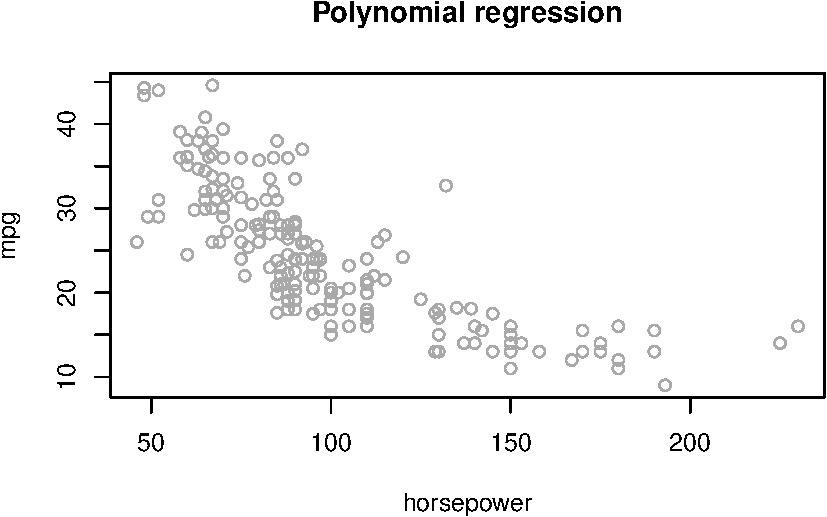
\includegraphics[width=0.7\linewidth]{RecEx11_files/figure-latex/unnamed-chunk-1-1} \end{center}

\begin{center}\rule{0.5\linewidth}{0.5pt}\end{center}

\hypertarget{a-2}{%
\subsubsection{a)}\label{a-2}}

Preprocessing is important before we fit a neural network. Standardize
the features and transform the digits to factors for both train and test
data.

Remember that it is important to decide on the scale based on the
training data, and then apply the same standardization for both training
and test data (i.e., centering around the same mean and transforming to
the same variance).

\hypertarget{b-2}{%
\subsubsection{b)}\label{b-2}}

One of the simplest ways of fitting simple neural networks in R is via
the \texttt{nnet()} function in the R package \texttt{nnet} (this was
not discussed in the lecture, but is useful to know anyway). Install the
package and check the help file typing \texttt{?nnet} into the console.

\begin{enumerate}
\def\labelenumi{(\roman{enumi})}
\item
  What is the main limitation of the \texttt{nnet()} function?
\item
  Use a feedforward-network with one hidden layer to train and predict
  using the \texttt{nnet()} function. Include 5 hidden nodes plus a bias
  node in the input and hidden layers. What is the number of parameters?
\item
  Look at the confusion table for the test data. How good does the
  network perfom?
\end{enumerate}

\hypertarget{problem-4-deep-learning-with-keras}{%
\section{Problem 4: Deep Learning with
Keras}\label{problem-4-deep-learning-with-keras}}

We again work on a handwritten digit recognition problem, but now we use
the data from the keras library. This dataset consists of 60000 training
data of \(28\times28\) grayscale images and 10000 test data.

For more info see \href{https://keras.rstudio.com/}{here:
https://keras.rstudio.com/}.

If you have already installed \texttt{keras} ignore the following chunk
of code

\begin{Shaded}
\begin{Highlighting}[]
\CommentTok{# Install the keras R package}
\KeywordTok{install.packages}\NormalTok{(}\StringTok{"keras"}\NormalTok{)}
\CommentTok{# Install the core Keras library + TensorFlow}
\KeywordTok{library}\NormalTok{(keras)}
\KeywordTok{install_keras}\NormalTok{()}
\CommentTok{# for machines with NVIDIA GPU install_keras(tensorflow = 'gpu')}
\end{Highlighting}
\end{Shaded}

\hypertarget{data-preprocessing}{%
\subsubsection{Data Preprocessing}\label{data-preprocessing}}

\begin{Shaded}
\begin{Highlighting}[]
\KeywordTok{library}\NormalTok{(keras)}
\NormalTok{mnist =}\StringTok{ }\KeywordTok{dataset_mnist}\NormalTok{()}
\NormalTok{x_train =}\StringTok{ }\NormalTok{mnist}\OperatorTok{$}\NormalTok{train}\OperatorTok{$}\NormalTok{x}
\NormalTok{y_train =}\StringTok{ }\NormalTok{mnist}\OperatorTok{$}\NormalTok{train}\OperatorTok{$}\NormalTok{y}
\NormalTok{x_test =}\StringTok{ }\NormalTok{mnist}\OperatorTok{$}\NormalTok{test}\OperatorTok{$}\NormalTok{x}
\NormalTok{y_test =}\StringTok{ }\NormalTok{mnist}\OperatorTok{$}\NormalTok{test}\OperatorTok{$}\NormalTok{y}

\CommentTok{# reshape}
\NormalTok{x_train =}\StringTok{ }\KeywordTok{array_reshape}\NormalTok{(x_train, }\KeywordTok{c}\NormalTok{(}\KeywordTok{nrow}\NormalTok{(x_train), }\DecValTok{28} \OperatorTok{*}\StringTok{ }\DecValTok{28}\NormalTok{))}
\NormalTok{x_test =}\StringTok{ }\KeywordTok{array_reshape}\NormalTok{(x_test, }\KeywordTok{c}\NormalTok{(}\KeywordTok{nrow}\NormalTok{(x_test), }\DecValTok{28} \OperatorTok{*}\StringTok{ }\DecValTok{28}\NormalTok{))}
\CommentTok{# rescale}
\NormalTok{x_train =}\StringTok{ }\NormalTok{x_train}\OperatorTok{/}\DecValTok{255}
\NormalTok{x_test =}\StringTok{ }\NormalTok{x_test}\OperatorTok{/}\DecValTok{255}

\NormalTok{y_train =}\StringTok{ }\KeywordTok{to_categorical}\NormalTok{(y_train, }\DecValTok{10}\NormalTok{)}
\NormalTok{y_test =}\StringTok{ }\KeywordTok{to_categorical}\NormalTok{(y_test, }\DecValTok{10}\NormalTok{)}
\end{Highlighting}
\end{Shaded}

\hypertarget{a-3}{%
\subsubsection{a)}\label{a-3}}

In order to fit a model in keras we can use the following steps. We fit
a densely (or fully) conected neural network with 2 hidden layers. Fill
in the missing inputs and run the model.

\hypertarget{define-the-model}{%
\subparagraph{1. Define the model}\label{define-the-model}}

\begin{Shaded}
\begin{Highlighting}[]
\NormalTok{model =}\StringTok{ }\KeywordTok{keras_model_sequential}\NormalTok{() }\OperatorTok\StringTok{ }
\StringTok{  }\KeywordTok{layer_dense}\NormalTok{(}\DataTypeTok{units =} \DecValTok{8}\NormalTok{, }\DataTypeTok{activation =} \StringTok{'relu'}\NormalTok{, }\DataTypeTok{input_shape =} \KeywordTok{c}\NormalTok{(...)) }\OperatorTok\StringTok{ }\CommentTok{# fill in the length of the input layer }
\StringTok{  }\KeywordTok{layer_dense}\NormalTok{(}\DataTypeTok{units =} \DecValTok{8}\NormalTok{, }\DataTypeTok{activation =} \StringTok{'relu'}\NormalTok{) }\OperatorTok
\StringTok{  }\KeywordTok{layer_dense}\NormalTok{(}\DataTypeTok{units =} \DecValTok{10}\NormalTok{, }\DataTypeTok{activation =}\NormalTok{ ...) }\CommentTok{# fill in the name of the activation function}
\end{Highlighting}
\end{Shaded}

Possible choices of the activation function are `sigmoid', `softmax' or
the identity function (which means that we don't have to define any
activation argument in the last layer). What is the use of identity
function?

\hypertarget{compile}{%
\subparagraph{2. Compile}\label{compile}}

\begin{Shaded}
\begin{Highlighting}[]
\NormalTok{model }\OperatorTok\StringTok{ }\KeywordTok{compile}\NormalTok{(}\DataTypeTok{optimizer =} \StringTok{"rmsprop"}\NormalTok{, }\DataTypeTok{loss =}\NormalTok{ ..., }\DataTypeTok{metrics =} \KeywordTok{c}\NormalTok{(...))}
\end{Highlighting}
\end{Shaded}

Possible choices of loss function are `binary\_crossentropy',
`categorical\_crossentropy' and `mse'. For metrics you can use
`mean\_absolute\_error' or `accuracy'.

\hypertarget{train}{%
\subparagraph{3. Train}\label{train}}

\begin{Shaded}
\begin{Highlighting}[]
\NormalTok{history =}\StringTok{ }\NormalTok{model }\OperatorTok\StringTok{ }\KeywordTok{fit}\NormalTok{(x_train, y_train, }\DataTypeTok{epochs =} \DecValTok{20}\NormalTok{, }\DataTypeTok{batch_size =} \DecValTok{128}\NormalTok{, }
    \DataTypeTok{validation_split =} \FloatTok{0.2}\NormalTok{)}
\end{Highlighting}
\end{Shaded}

You can find more information about the different arguments in the
\texttt{fit()} function here:
\url{https://keras.rstudio.com/reference/fit.html}

Report the accuracy on the test data.

\begin{Shaded}
\begin{Highlighting}[]
\KeywordTok{str}\NormalTok{(history)}
\KeywordTok{plot}\NormalTok{(history)}
\NormalTok{model }\OperatorTok\StringTok{ }\KeywordTok{evaluate}\NormalTok{(x_test, y_test)}
\end{Highlighting}
\end{Shaded}

What is the number of parameters?

\hypertarget{b-3}{%
\subsubsection{b)}\label{b-3}}

Now fit a model with 2 hidden layers with 128 units each. What do you
see?

\hypertarget{c-2}{%
\subsubsection{c)}\label{c-2}}

In order to avoid the problem we have seen in b), we can use weight
reguralization (L1 and L2 norms) or dropout. Apply these methods to the
network from b).

\textbf{R-hint:} for weight reguralization you can use

\begin{Shaded}
\begin{Highlighting}[]
\KeywordTok{layer_dense}\NormalTok{(}\DataTypeTok{units =} \DecValTok{16}\NormalTok{, }\DataTypeTok{activation =} \StringTok{"relu"}\NormalTok{, }\DataTypeTok{input_shape =} \DecValTok{28}\OperatorTok{*}\DecValTok{28}\NormalTok{, }
            
            \DataTypeTok{kernel_regularizer =} \KeywordTok{regularizer_l2}\NormalTok{(}\DataTypeTok{l =} \FloatTok{0.001}\NormalTok{))}
\end{Highlighting}
\end{Shaded}

and for dropout you can use
\texttt{layer\_dropout(0.5)\ \%\textgreater{}\%} after each hidden
layer. For more details see
\href{https://keras.rstudio.com/articles/tutorial_overfit_underfit.html}{here}.

\hypertarget{d-1}{%
\subsubsection{d)}\label{d-1}}

Now, let's try using convolutional neural network (CNN) instead of
densely(fully)-connected neural network (DNN). We're building a CNN
model that consists of three convolutional layers with the max pooling
layers. The convolutional layers are followed by the flatten layer and
dense layer. For more information, you can refer to
\href{https://tensorflow.rstudio.com/tutorials/advanced/images/cnn/}{here}.

The 2nd following code script builds the CNN model and its number of
trainable parameters are almost the same as that of the DNN model shown
in a) so that we can compare the performance difference between the DNN
model and the CNN model when their model size (i.e., number of trainable
parameters) are the same. Fill in the missing inputs and run the model.

\begin{Shaded}
\begin{Highlighting}[]
\CommentTok{# re-define `x_train`, ..., `y_test` to keep them as 2-dimensional.}
\NormalTok{mnist =}\StringTok{ }\KeywordTok{dataset_mnist}\NormalTok{()}
\NormalTok{x_train =}\StringTok{ }\NormalTok{mnist}\OperatorTok{$}\NormalTok{train}\OperatorTok{$}\NormalTok{x}
\NormalTok{y_train =}\StringTok{ }\NormalTok{mnist}\OperatorTok{$}\NormalTok{train}\OperatorTok{$}\NormalTok{y}
\NormalTok{x_test =}\StringTok{ }\NormalTok{mnist}\OperatorTok{$}\NormalTok{test}\OperatorTok{$}\NormalTok{x}
\NormalTok{y_test =}\StringTok{ }\NormalTok{mnist}\OperatorTok{$}\NormalTok{test}\OperatorTok{$}\NormalTok{y}

\CommentTok{# rescale}
\NormalTok{x_train =}\StringTok{ }\NormalTok{x_train}\OperatorTok{/}\DecValTok{255}
\NormalTok{x_test =}\StringTok{ }\NormalTok{x_test}\OperatorTok{/}\DecValTok{255}

\NormalTok{y_train =}\StringTok{ }\KeywordTok{to_categorical}\NormalTok{(y_train, }\DecValTok{10}\NormalTok{)}
\NormalTok{y_test =}\StringTok{ }\KeywordTok{to_categorical}\NormalTok{(y_test, }\DecValTok{10}\NormalTok{)}
\end{Highlighting}
\end{Shaded}

\begin{Shaded}
\begin{Highlighting}[]
\CommentTok{# define a CNN model}
\NormalTok{model <-}\StringTok{ }\KeywordTok{keras_model_sequential}\NormalTok{() }\OperatorTok\StringTok{ }\KeywordTok{layer_conv_2d}\NormalTok{(}\DataTypeTok{filters =} \DecValTok{8}\NormalTok{, }\DataTypeTok{kernel_size =} \KeywordTok{c}\NormalTok{(}\DecValTok{3}\NormalTok{, }
    \DecValTok{3}\NormalTok{), }\DataTypeTok{activation =} \StringTok{"relu"}\NormalTok{, }\DataTypeTok{input_shape =} \KeywordTok{c}\NormalTok{(...)) }\OperatorTok\StringTok{ }\KeywordTok{layer_max_pooling_2d}\NormalTok{(}\DataTypeTok{pool_size =} \KeywordTok{c}\NormalTok{(}\DecValTok{2}\NormalTok{, }
    \DecValTok{2}\NormalTok{)) }\OperatorTok\StringTok{ }\KeywordTok{layer_conv_2d}\NormalTok{(}\DataTypeTok{filters =} \DecValTok{16}\NormalTok{, }\DataTypeTok{kernel_size =} \KeywordTok{c}\NormalTok{(}\DecValTok{3}\NormalTok{, }\DecValTok{3}\NormalTok{), }\DataTypeTok{activation =} \StringTok{"relu"}\NormalTok{) }\OperatorTok\StringTok{ }
\StringTok{    }\KeywordTok{layer_max_pooling_2d}\NormalTok{(}\DataTypeTok{pool_size =} \KeywordTok{c}\NormalTok{(}\DecValTok{2}\NormalTok{, }\DecValTok{2}\NormalTok{)) }\OperatorTok\StringTok{ }\KeywordTok{layer_conv_2d}\NormalTok{(}\DataTypeTok{filters =} \DecValTok{22}\NormalTok{, }
    \DataTypeTok{kernel_size =} \KeywordTok{c}\NormalTok{(}\DecValTok{3}\NormalTok{, }\DecValTok{3}\NormalTok{), }\DataTypeTok{activation =} \StringTok{"relu"}\NormalTok{) }\OperatorTok\StringTok{ }\KeywordTok{layer_flatten}\NormalTok{() }\OperatorTok\StringTok{ }
\StringTok{    }\KeywordTok{layer_dense}\NormalTok{(}\DataTypeTok{units =} \DecValTok{10}\NormalTok{, }\DataTypeTok{activation =}\NormalTok{ ...)}
\KeywordTok{summary}\NormalTok{(model)}
\end{Highlighting}
\end{Shaded}

\begin{Shaded}
\begin{Highlighting}[]
\CommentTok{# run}
\NormalTok{model }\OperatorTok\StringTok{ }\KeywordTok{compile}\NormalTok{(}\DataTypeTok{optimizer =} \StringTok{"rmsprop"}\NormalTok{, }\DataTypeTok{loss =} \StringTok{"categorical_crossentropy"}\NormalTok{, }
    \DataTypeTok{metrics =} \KeywordTok{c}\NormalTok{(}\StringTok{"accuracy"}\NormalTok{))}

\NormalTok{history =}\StringTok{ }\NormalTok{model }\OperatorTok\StringTok{ }\KeywordTok{fit}\NormalTok{(x_train, y_train, }\DataTypeTok{epochs =} \DecValTok{20}\NormalTok{, }\DataTypeTok{batch_size =} \DecValTok{128}\NormalTok{, }
    \DataTypeTok{validation_split =} \FloatTok{0.2}\NormalTok{)}

\KeywordTok{str}\NormalTok{(history)}
\KeywordTok{plot}\NormalTok{(history)}
\end{Highlighting}
\end{Shaded}

\end{document}
